\documentclass[a4paper,12pt]{article}
\usepackage[utf8]{inputenc}
\usepackage[T1]{fontenc}
\usepackage[sorting=nyt,citestyle=authoryear]{biblatex}
\addbibresource{report.bib}
\usepackage[normalem]{ulem}
\usepackage{hyperref}
\usepackage{libertine}
\usepackage[scaled=0.89]{inconsolata}
\usepackage[showframe=false,bottom=6em,head=8em]{geometry}
\usepackage[iso,danish]{isodate}
\usepackage{fancyvrb}
\usepackage{fancyhdr}
\usepackage{fancyref}
\usepackage{float}
\usepackage{tikz}
\usetikzlibrary{arrows.meta}
\usepackage{pgfplots}
\pgfplotsset{compat=1.15}
\usepackage{amsmath}

\pagestyle{fancy}
\fancyhf{}
\lhead{FF501 Consensus in Distributed Systems}
\rhead{\today}
\chead{}
\lfoot{J. R. Fagerberg, M. Møller, L. O. J. Olsen, P. H. Ratgen, T. Stenhaug}
\cfoot{}
\rfoot{\thepage}
\renewcommand{\footrulewidth}{0pt}
\setcounter{secnumdepth}{2}
\setcounter{tocdepth}{2}

\date{\today}
\title{FF501 Consensus in Distributed Systems}
\author{
  Johan Ringmann Fagerberg \\
  Marcus Møller \\
  Lucas Olai Jarlkov Olsen \\
  Peter Heilbo Ratgen \\
  Thomas Stenhaug
}

\pagenumbering{roman}

\begin{document}

\maketitle

\setlength{\baselineskip}{1.44\baselineskip}

\begin{abstract}

Clock synchronization is a widely known problem that has many applications. E.g. multiple clients in a distributed system must agree on a single time in order to successfully tackle a problem. The problem has been worked on since the birth of computer networks, and solutions have evolved over time in response to changing demands. In recent years, consensus based algorithms have gained traction with the propagation of Internet of Things, and several new algorithms have been developed as a result.

We will compare two recent consensus-based algorithms for clock synchronization in distributed systems, Average TimeSync (ATS) and Maximum Minimum Time Sync (MMTS), and implement them. The comparison will be based on the theoretical work from the algorithms' authors, our own analysis, and an implementation of both algorithms in virtual distributed networks.
\end{abstract}

\clearpage
\tableofcontents
\clearpage

\pagenumbering{arabic}
\setcounter{page}{1}

\section{Preface}

\section{Introduction (WIP)}

\subsection{Distributed systems}

A definition of \textit{distributed system} is
\begin{quote}
  A distributed system is a collection of autonomous computing
  elements that appears to its users as a single, coherent
  system.\cite{TanenbaumSteen06}
\end{quote}

The computing elements are typically called
nodes \cite{TanenbaumSteen06}, which is the term we will use within.
Nodes can be both hardware units, of software processes, while
\textit{users} might refer both to humans and software processes.

An example of a distributed system is a multi-player online game, where
the game environment is experienced as a single system, while there
are several nodes concerting the unified experience.  Another example
is the World Wide Web, which you can view as a large key-value store,
where Uniform Resource Locatiors (URL) are the key, and (typically)
HTML-pages are their value.  In the case of the WWW, both humans and
processes can considered users; indexing crawlers like Google are
examples of computer process users.  The type of distributed systems
we have studied, are \textit{Wireless Sensor Network}s (WSN), which is
discussed further below.

The type of distributed systems we have studied, are wireless sensor
networks.  Here, the nodes are small, cheap devices, equipped with the
ability to monitor environmental variables, like temperature,
humidity, sound pollution and so on. [cite?]

\subsection{Consensus}

Autonomous nodes that are to appear as a single system must share some
state.  For contrast, systems where there are master and slave nodes,
synchronization of shared data is achieved by pushing data from the
master to the slaves.  When nodes are ``peers'', consensus must be
reached by other means, and it must be reached in the face of faulty
or malicious nodes.

An example of faults, \textit{Byzantine faults}, were described in
Lamport, Shostak and Pease in a 1982 paper \cite{Lamport82}.  A group
of Byzantine generals, each general commanding a division, is
besieging a city.  They must reach an agreement on whether to all
attack or all retreat, and they can only communicate through messages.
There might be traiterous generals (faulty nodes), which send
different messages to different generals while loyal generals always
send the same message to all generals.

\subsection{Clock Synchronization}

There is not really a global clock in distributed systems.  In WSNs in
particular, it is too expensive to have an atomic clock at every node.

Depending on the application of the distributed system, different
``levels'' of synchronization might be chosen.  

Logical clocks \cite{Lamport78}, are chosen when it's only the strong
ordering of events within the system that is necessary.  If $c(x)$ is
a function of the system's ``clock'' at the point when event $x$.  Using
$a \rightarrow b$ to mean $a$ precedes $b$, then the strong clock condition is that
$a \rightarrow b \Rightarrow c(a) \rightarrow c(b)$

[TDSM, sync with atomic, prior protocols?]

\section{Theory}

\subsection{Time synchronization} % Mostly done, might need to be split up

%Describe the time synchronization problem. Why is it necessary? Why is it not trivial?

Time synchronization is the problem of having a network of nodes agree on the value of their local clock at a given instant. It is an important part of any distributed system that requires some level of sequentiality of events; examples include banks, where the order of withdrawing and depositing is important, sharded databases, where the order of insertions, modifications and deletions is important, and even our daily lives, where a shared clock is important for meeting and scheduling with other people.

There are many different variants of the time synchronization problem, each with their own goals and disadvantages.

The most intuitive is the propagation of a "true" time throughout a network, as happens with our electronic devices today. For this approach one or more high-precision clock are seen as authoritative, and the value reported by them is propagated throughout the network and accepted at each node as the absolute truth. Unfortunately this is fragile to failed or malicious nodes near the root level. It is nonetheless the problem that must be solved if a known time must be propagated throughout the network.

An alternative problem is reaching consensus on a shared time in a network, regardless of what said time is. This is useful for ensuring sequentiality of events within the network, and can be made highly resistant to failed or malicious nodes in the network, as no nodes have a greater weight than others when it comes to reaching consensus on a value. As such this problem is highly applicable to scenarios where the reliability of the consensus is important, and where the impact of nodes joining or leaving the network must be limited. It is primarily this problem we will be discussing in this paper.


\subsubsection{Clock modelling}
%Clock drift

The hardware clock available to each node is often a low precision clock, whose time progression rate is not necessarily equal to that of other clocks. This means that over time, the output of the hardware clock will slowly drift away from other clocks. As the clock may have drifted considerably before the clock is observed, this also results in an initial time offset.

For the sake of modelling such a clock the concept of a virtual absolute time $t$ is introduced. This time is not known to any nodes, but is a useful tool, as it allows us to express the output of a given clock as a function of the current absolute time.

As such the local hardware clock $\tau$ of a node $i$ can be modelled as a linear function with two parameters, the skew $\alpha$ and the offset $\beta$:

\begin{equation}\label{eq:hardware-clock}
    \tau_i(t) = \alpha_i t + \beta_i.
\end{equation}

It is important to note that as $t$ is not known, neither $\alpha$ nor $\beta$ can be calculated directly. The only aspect of the hardware clock visible to the node is the output $\tau(t)$.

As the goal of clock synchronization is to find a way for every node in a network to report the same time at a given $t$ despite differing hardware clocks, equation \ref{eq:hardware-clock} must be transformed into a function that can be modified by the node. For this reason, the concept of logical clocks $L$ is introduced, defined as

\begin{align}
    L_i(t) &= \hat\alpha_i \tau_i(t) + \hat\beta_i \nonumber \\
        &= \hat\alpha_i \alpha_i t + \hat\alpha_i \beta_i + \hat\beta_i. \label{eq:logical-clock-expanded}
\end{align}

Modifying $\hat\alpha_i$ and $\hat\beta_i$ allows the node to change the output of the logical clock in relation to $t$, without knowing the parameters of the hardware clock $\tau$.

The goal of reaching consensus can thus be formalized in terms of logical clocks: As equation \ref{eq:logical-clock-expanded} makes clear, having two logical clocks $L_i$ and $L_j$ agree on the output at a given $t$ means having the parameters $\hat\alpha_i \alpha_i \approx \hat\alpha_j \alpha_j$ and $\hat\alpha_i \beta_i + \hat\beta_i \approx \hat\alpha_j \beta_j + \hat\beta_j$. Note that this does not mean that $\hat\alpha_i \approx \hat\alpha_j$, nor that $\hat\beta_i \approx \hat\beta_j$, as the parameters of the hardware clocks are likely to differ.

Expanding this to the entire network, reaching consensus can be formalized as reaching the point where $\hat\alpha_i \alpha_i \approx A$ and $\hat\alpha_i \beta_i + \hat\beta_i \approx B$, with $A$ and $B$ being network-global constants, for every node $i$ in the network.

%Time sync in 

\subsection{Strategies for time synchronization (WIP(Peter))}

%Describe the advantages and disadvantages of the different kinds of time synchronization strategies (non-consensus vs. consensus)
By in-large there are two ways of approaching the time synchronization problem, these being consensus and non-consensus based algorithms.

    \subsubsection{Non-consensus}
    %In general about non-consensus
    Examples of non-consensus time synchronization algorithms are The Berkeley algorithm, Reference Broadcast Synchronization (RBS) and The Flooding Time Sync Protocol (FTSP). All of these algorithms incorporate some form of master-slave relationship. Regarding RBS and FTSP, these are tailored to Wireless Sensor Networks (WSN).
    
    %Not sure if it should be included
    \paragraph{The Berkeley algorithm} The simplest algorithms is the Berkeley algorithm (\cite{Gusella89}), it works by having a centralized time server polling the nodes for their current clock value. The time server then averages these clock values, along with its own clock value. The time server then tells each node to adjust to the averaged clock value. 
    
    %\paragraph{NTP}
    
    \paragraph{RBS} The Reference Broadcast algorithm, described by \cite{ElsonGirodEstrin02},  functions by a central node sending out a reference packet to each node. Each node then records the time at which the reference packet was received. %Exhanging of recorded clock times? 
    The nodes should then compare their results. This is done by calculating their offset relative to another receiver. The offset is calculated by 
    \begin{equation}
        \label{offsetcalc}
        \textit{Offset} [i,j] = \frac{1}{M}\sum^M_{k=1} (T_{j,k} - T_{i,k})
    \end{equation}
    where $i$ and $j$ are two nodes and $T_{p,a}$ is $p$'s clock when it received broadcast $a$. $M$ is the number of reference broadcasts.  %Handling of clock skew.
    However calculating the offset of a node's clock relative to another, and vice versa is not enough as it doesn't take clock drift into account. However this can be solved by using linear regression to get the offset as a function.
    $$\textit{Offset}[i,j](t) = \alpha t + \beta$$
    This allows for a more accurate estimation of a nodes current clock value by another node.
    
    %Post-facto synchronization
    
    \paragraph{TPSN} The Timing-sync Protocol for Sensor Networks protocol, described by \cite{GaneriwalEtAl03}, functions by selecting a node as the root node. At first the algorithm enters the "level discovery phase", in this  phase each node is assigned a level. This is done the root node sending out a \texttt{level\_discovery} packet. Then each node assigns itself to a level lower than from which at received the packet. This node then broadcasts a \texttt{level\_discovery}. The algorithms then enters the synchronization phase, it uses sender-receiver synchronization. This sets it apart from RBS, which uses receiver-receiver synchronization. This mean that the receiver synchronizes to the sender. The time is synchronized by calculating the clock drift and the propagation time between nodes. As seen on figure \ref{timemeasuretpsn}, the receiver node A sends a synchronization pulse to the sender B, which is located at a greater level. Node A sends a synchronization pulse to B, which in turn sends back an acknowledgement packet. This acknowledgement packet contains the values of $T_1$, $T_2$ and $T_3$. Then the final time $T_4$ is recorded by node A. From these values the clock drift ($\Delta$) and propagation delay ($d$) between the two nodes can be calculated. 
    
    $$\Delta = \frac{(T_2-T_1) - (T_4 - T_3)}{2} \quad ; \quad d = \frac{(T_2-T_1) + (T_4-T_3)}{2}$$
    
    \begin{figure}[H]
        \centering
        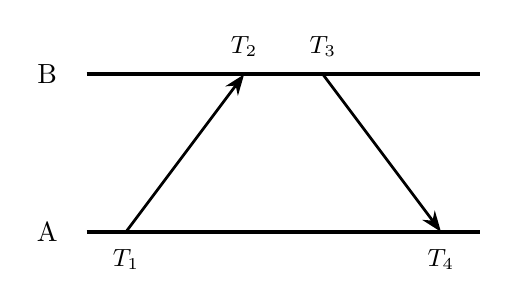
\begin{tikzpicture}
            \draw [line width = 1.5pt](0,0) node (upper-line-start){}
                  -- (5,0) node (upper-line-end){};
            \draw [line width = 1.5pt](0,-2) node (lower-line-start){}
                  -- (5,-2) node (lower-line-end){};
            \node [left of = upper-line-start, node distance = 0.5cm](){B};
            \node [left of = lower-line-start, node distance = 0.5cm](){A};
            \draw [arrows={-Stealth[length = 7.5pt]}, line width = 1pt] (0.5,-2) node (first-line-start){}
                  -- (2,0) node (first-line-end){};
            \draw [arrows={-Stealth[length = 7.5pt]}, line width = 1pt] (3,0) node (last-line-start){}
                  -- (4.5,-2) node (last-line-end){};
            \node [below of = first-line-start, node distance = 0.35cm] (){\small $T_1$};
            \node [above of = first-line-end, node distance = 0.35cm] (){\small $T_2$};
            \node [above of = last-line-start, node distance = 0.35cm] (){\small $T_3$};
            \node [below of = last-line-end, node distance = 0.35cm] (){\small $T_4$};
         \end{tikzpicture}
         \caption{A model of communication between nodes. $T_1$ and $T_4$ are recorded on the clock of node A, and $T_2$ and $T_3$ on the clock of node B}
        \label{timemeasuretpsn}
    \end{figure}
    
    In general the synchronization is initiated by the root node. By instructing level 1 nodes to synchronize to the root node. When the level 1 nodes are synchronized, the level 2 nodes are synchronized and so forth. 
    
    %Level discovery and hierarchical structure
    %
    
    \paragraph{FTSP} %allegedly one of the best non-consensus algorithms
    
    The Flooding Time Sync Protocol, described by \cite{Maroti04}
    
    \subsubsection{Consensus}
    %In general about consensus based algorihms
    
    

%Describe algorithms Average TimeSync and Modified Maximum Time Sync.

\section{Analysis}%Or comparison
To analyze each of the two aforementioned Synchronization protocols we first researched their creation and how each of them function. What follows in this section is a short description of each of the protocols, Average Time Synchronization (ATS) and Modified Maximum Time Synchronization (MMTS). We'll describe how they function and discuss their advantages and disadvantages in certain situations and areas of application as well as their performance in an implemented simulated Wireless Sensor Network. Their performance will be compared on their synchronization accuracy and speed in the simulation.

%Perhaps have the description of the consensus algorithms in the previous section.

%Analyze the consensus-based algorithms Average TimeSync and Modified Maximum Time Sync. 
%Compare the algorithms, their advantages and disadvantages, and their areas of application (through both %implementation and theoretical analysis).

\subsection{Average Time Synchronization Protocol}



\section{Results}


\section{Discussion}

\section{Process analysis}%Not supposed to be in the report. Needs to be a separate document.

\section{Conclusion}



%\nocite{*} % print all bibliography, remove when actual citations are in place
\printbibliography


\end{document}